\chapter{基于变长语音段的情感识别}
\label{cha:var_len}

\section{本章引论}
\label{sec:var_len_intro}

上一章我们介绍了基于深度神经网络的端到端的语音情感识别系统,但是为了方便神经网络模型处理,一个完整的语音句子被切分成了更小的等长语音段,每一个语音段都被标记为对应句子的情感类别。这样的处理方式会引入一些问题,因为在我们实际的观测中,一个非中性的句子中并不是所有的语音段都会包含有明显的情感信息,往往只有一部分语音段包含情感信息。当我们将句子切分成多个语音段时,可能并不是所有的语音段都包含有情感信息,但在上一章的处理办法中仍然会将不包含情感信息的语音段标记为句子的情感类别。这样的数据在训练模型时会对模型造成混淆,因为同样的中性语音段,有的被标记为中性,有的被标记为其他情感,使得模型无法区分哪些应该是真正的中性语音。除了对中性情感的识别会产生影响以外,由于在预测时是由句子划分的所有语音段共同来决定句子最终的情感类别,而中性语音段对当前句子的情感区分贡献不大,所以也有可能会导致在识别时不同情感之间发生混淆。

一般而言,一个句子中只有部分语音含有明显的情感信息,为了进一步验证这一猜测,图\ref{fig:angry_spectrogram}展示了一个标记为愤怒的句子中前后两个语音段的语谱图,其中横轴代表时间,纵轴代表频率,颜色越深代表能量越高,(a)属于句子前半部分,(b)属于句子后半部分。

\begin{figure}[htb]
    \vspace{-0cm}  %调整图片与上文的垂直距离
    \setlength{\belowcaptionskip}{0cm}   %调整图片标题与下文距离
    \begin{minipage}{0.48\textwidth}
        \centering
        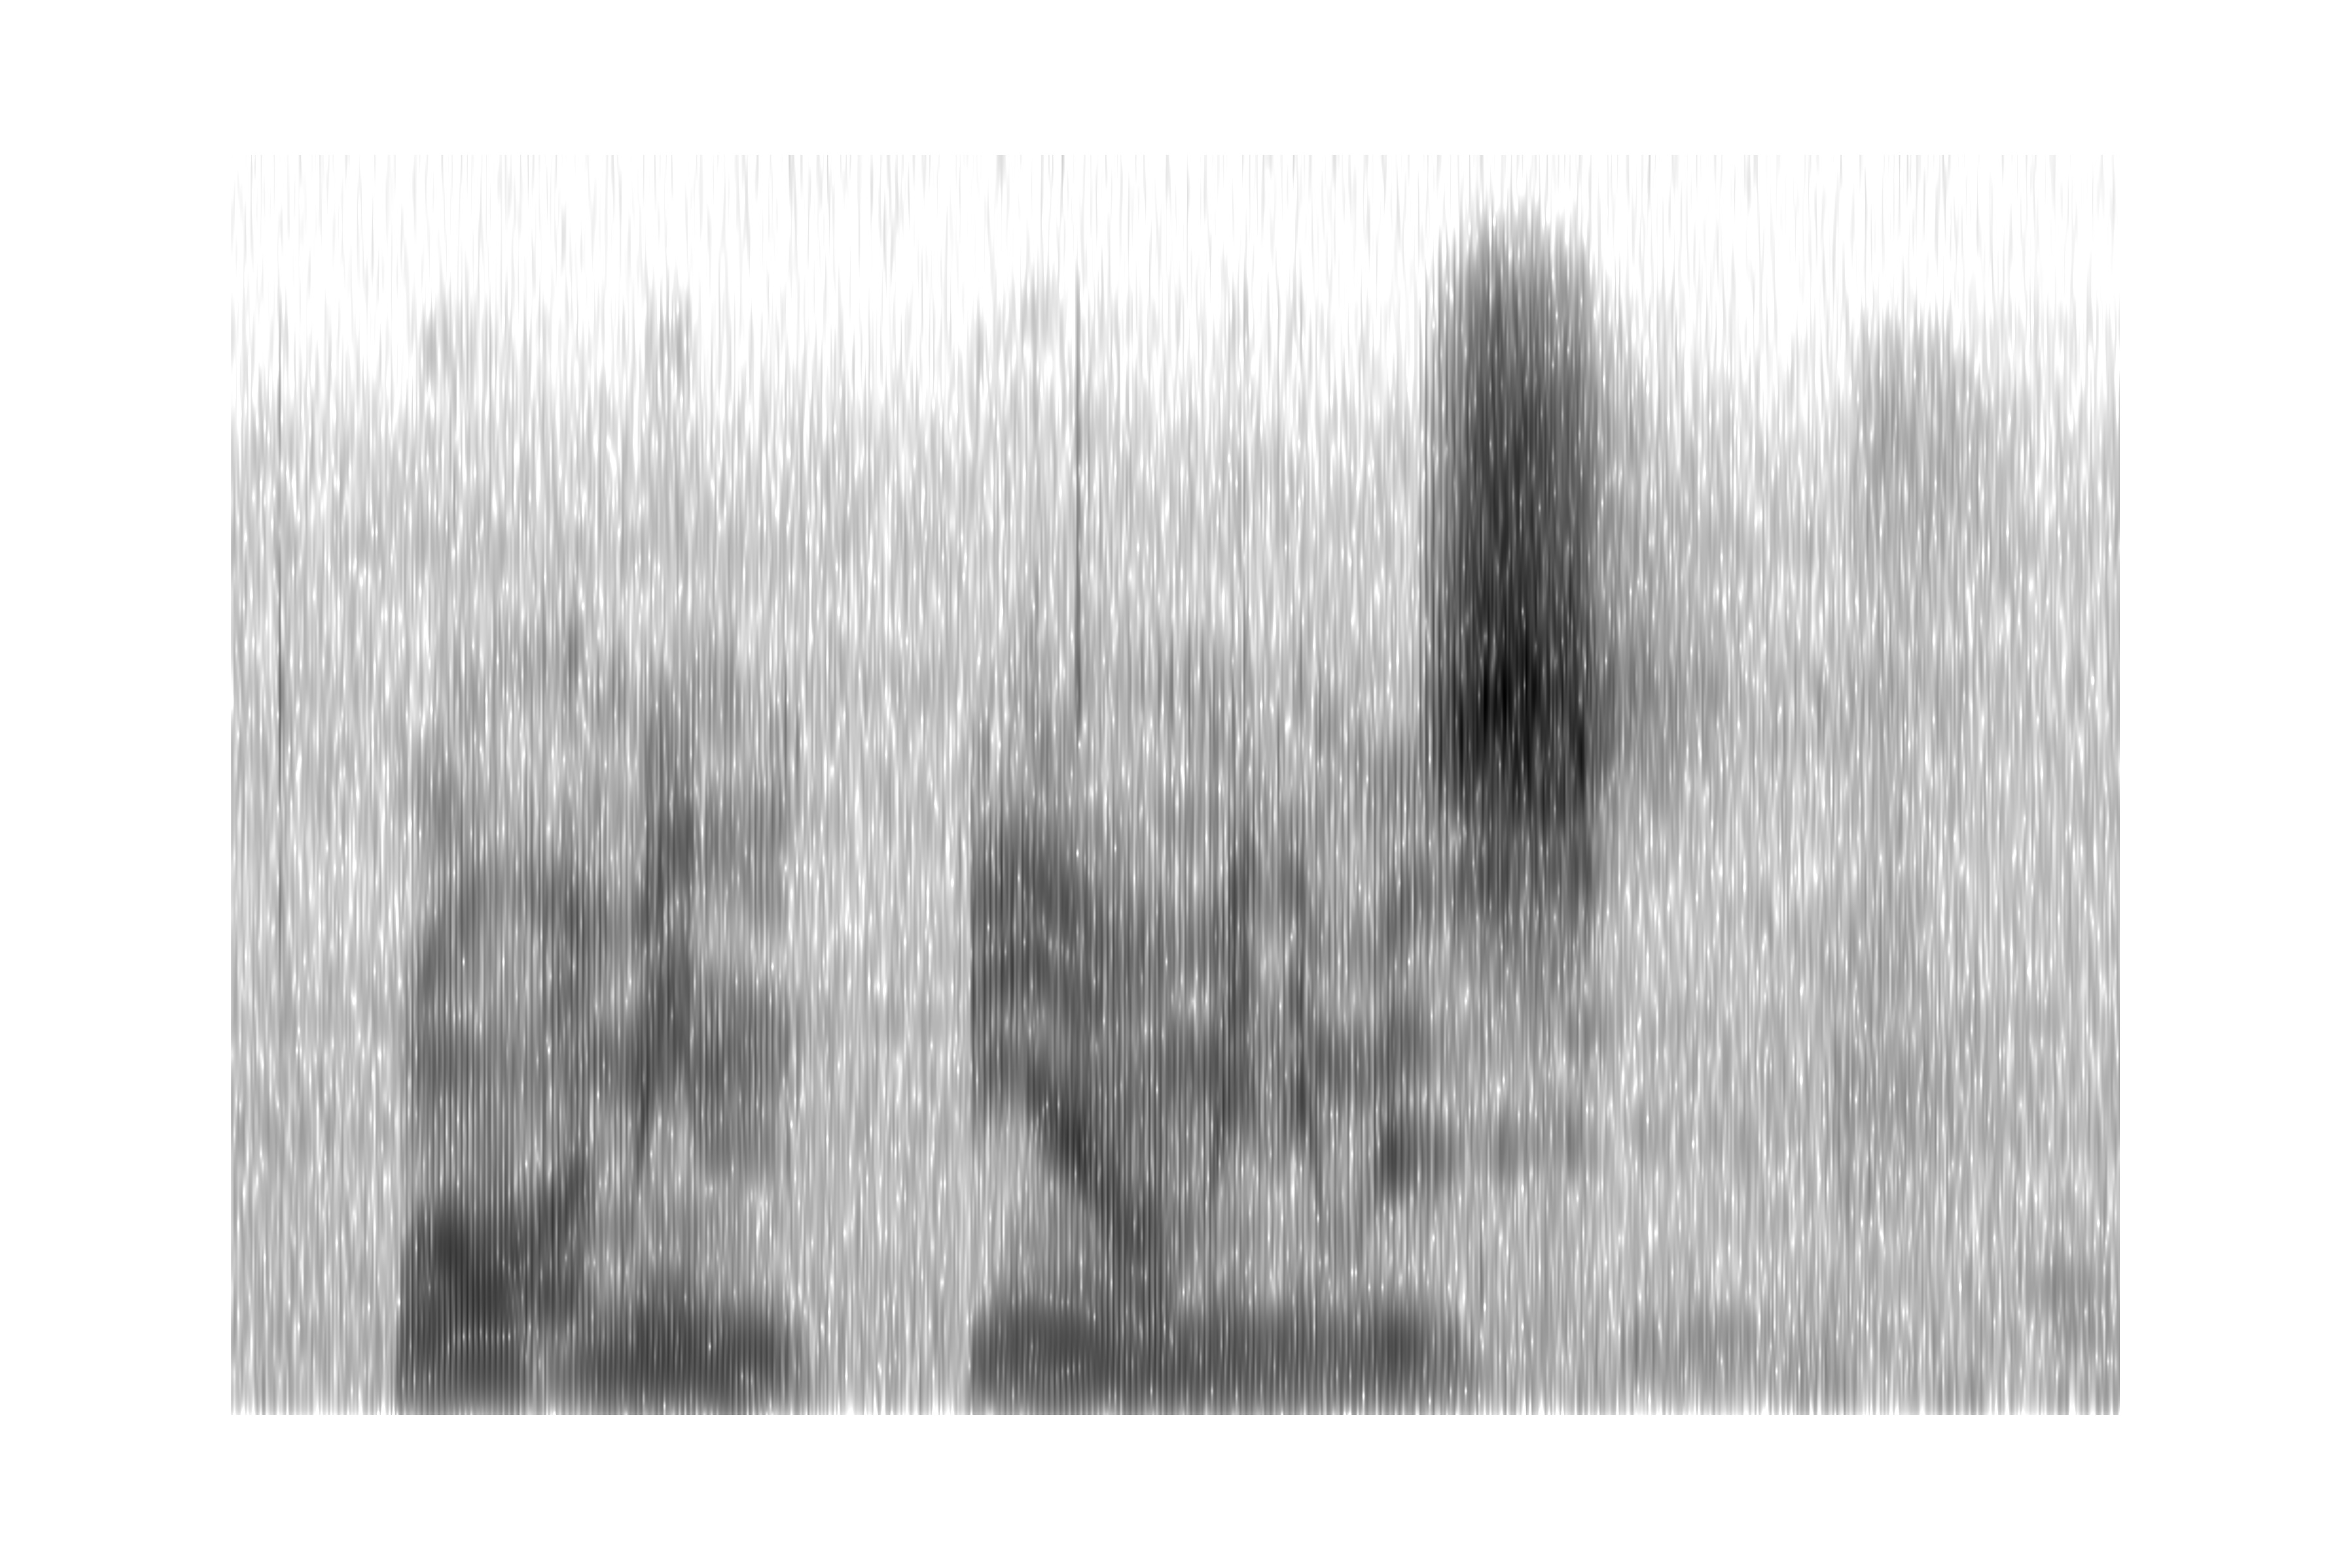
\includegraphics[height=5cm]{myfigures/angry_spectrogram_weak}
        \centerline{(a) 情感信息弱}\medskip
    \end{minipage}\hfill
    \begin{minipage}{0.48\textwidth}
        \centering
        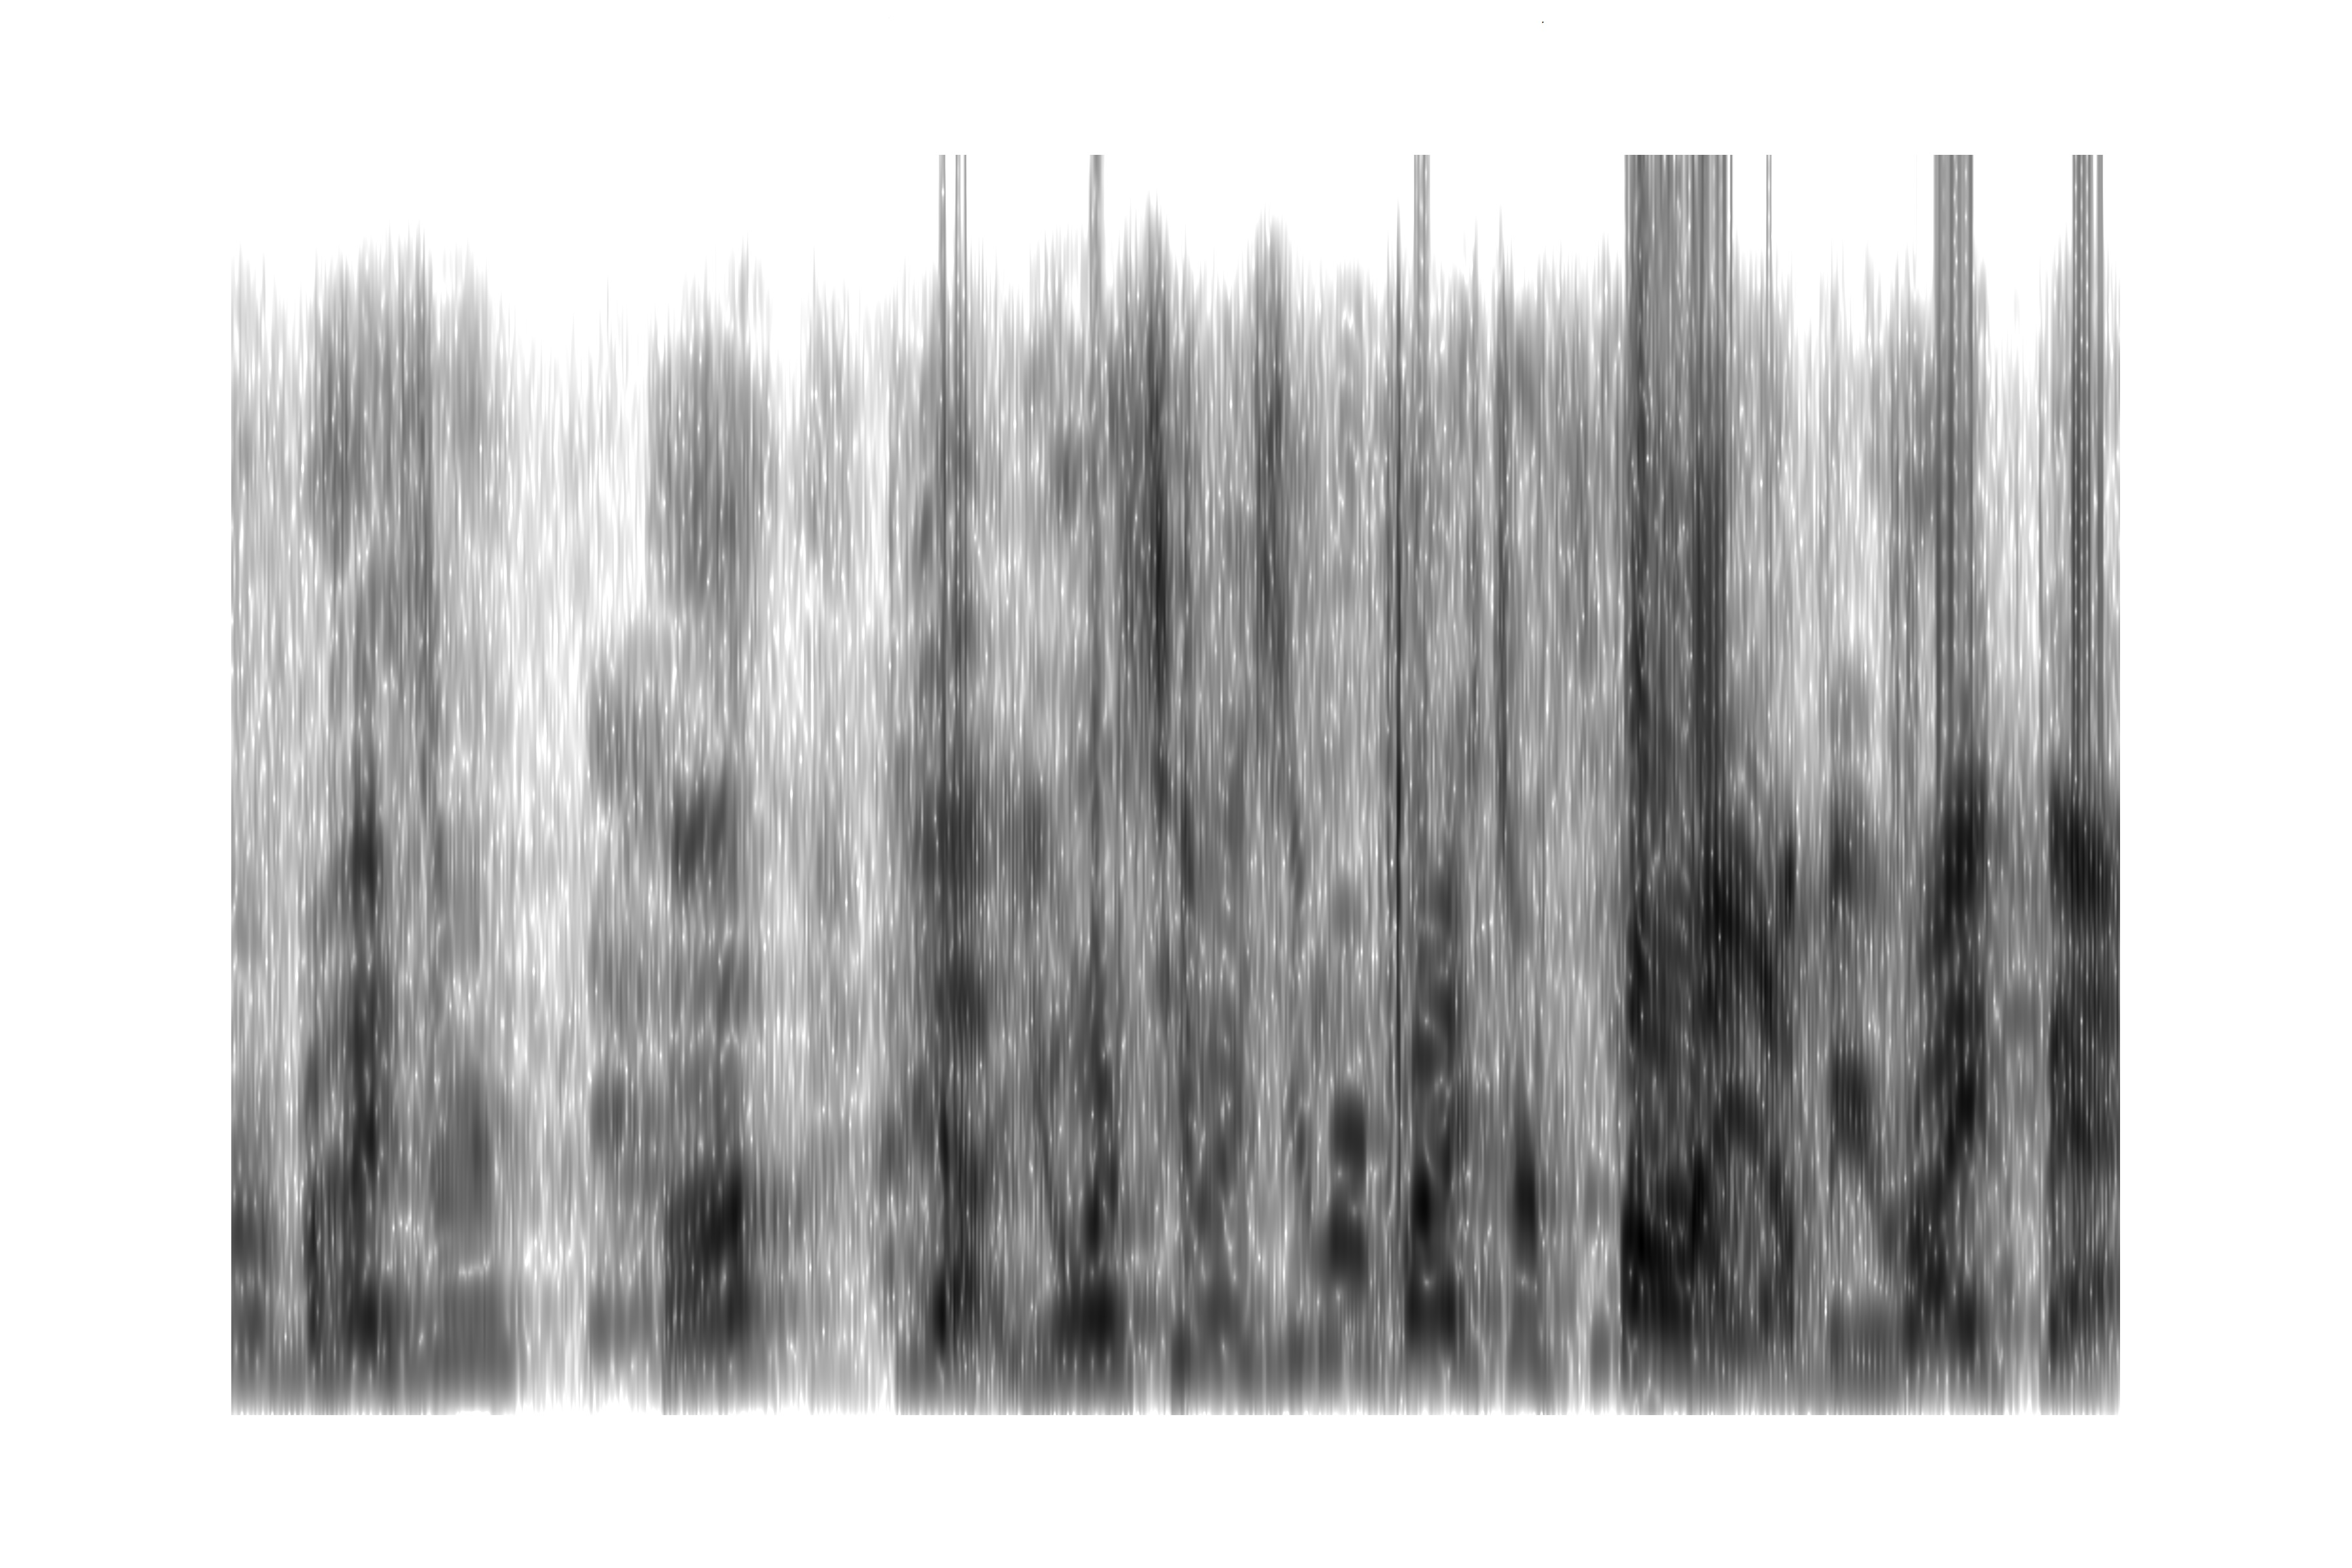
\includegraphics[height=5cm]{myfigures/angry_spectrogram_strong}
        \centerline{(b) 情感信息强}\medskip
    \end{minipage}
    \caption{愤怒句子不同语音段的语谱图}
    \label{fig:angry_spectrogram}
\end{figure}

通常来说,愤怒的语音在各个频段的能量都相对较高,可以看到图\ref{fig:angry_spectrogram}中(b)的语音段的能量较高,看上去更像一段愤怒的语音,而(a)的语音段则看上去却不像愤怒语音。通过人工听测这两个语音段,同样也发现(b)的语音段听上去包含有更多的愤怒情感,(a)的语音段听上去却更像中性语音。然而,当我们直接听整个句子时,却发现前面的中性语音段可以增强后面的愤怒语音段的愤怒感觉,也就是所谓的欲扬先抑。所以有必要将一个句子作为整体输入来进行情感识别。但是句子的长度通常都是不相同的,所以需要设计一种可以处理变长语音段的神经网络结构,并将整个句子作为输入以提升模型的识别率。

本章剩余的部分是这样安排的:首先我们将介绍变长语音段如何抽取语谱图和预处理,然后将介绍如何实现能够处理变长输入的深度神经网络模型,接下来将通过实验比较定长输入的神经网络和变长输入的神经网络在识别效果上的差异,以及分析定长模型和变长模型在相同语音输入的情况下神经网络的激活输出,最后总结本章的内容。

\section{变长语音段的语谱图抽取}

本章采取的语谱图抽取参数和上一章相同,唯一不同的是我们将对整个句子进行语谱图抽取,而不是对切分的等长语音段。由于在进行神经网络训练时,通常会将多个样本组成一个批次(Batch),然后一起放进训练算法去调整模型,并要求一个批次中的数据长度需要相同,但不同长度的句子得到的语谱图的长度各不相同,所以需要通过将一个批次中的语谱图都用0补齐到最长语谱图的长度。为了提升计算效率,所有的语谱图将会按照时间长度进行排序,然后将时间长度接近的语谱图放入一个批次,这样可以保证需要补齐的0最少,从而可以节约存储空间,提升计算速度。

\section{变长神经网络结构}
\label{sec:var_len_nn}

在上一章基于深度神经网络的端到端的语音情感识别系统中,我们主要采用了两种神经网络结构:卷积神经网络(Convolution Neutral Network, CNN)和循环神经网络(Recurrent Neural Network, RNN)。这两种神经网络结构通常的用法都是处理定长的输入,但它们同样也具备处理变长输入的能力。为了方便描述,假设输入序列为$\mathbf{s} = \{x_1, x_2,...,x_V,...,x_T\}$,其中$\mathbf{s}1 = \{x_1, x_2,...,x_V\}$是有效的部分,$\mathbf{s}2 = \{x_{V+1}, x_{V+2},...,x_T\}$是补齐的0。我们设计变长神经网络结构的主要目的就是不让补齐的0对最终的结果产生影响,下面将介绍本文是采用什么方法来设计模型,保证CNN和RNN都能够接受变长的输入,并且。

\subsection{变长卷积神经网络}
\label{ssec:var_len_cnn}

卷积神经网络(Convolution Neutral Network, CNN)是通常是处理定长的输入,特别是在计算机视觉领域。但实际上CNN本身只是在训练卷积核,而这些卷积核和输入的大小是无关的,因此CNN具备处理变长输入的能力。为了只保留有效的输入$\mathbf{s}1$对输出结果的影响,我们将采用掩码(Masking)去屏蔽补齐的无效输入$\mathbf{s}2$所产生的输出,如下面的公式所示:
\begin{equation}
\label{equ:cnn_mask}
    \mathbf{s}_{Conv} = Conv(\mathbf{s}) \bullet Mask(\mathbf{s})
\end{equation}
其中$Conv(\mathbf{s})$代表序列$s$在经过卷积层后的输出,$Mask(\mathbf{s})$代表掩码矩阵,矩阵中代表有效部分的位置被置为1,无效部分的位置被置为0,最终的有效输出为$\mathbf{s}_{Conv}=\{y1,y2,...,y_V,....,y_T\}$,是$Conv(\mathbf{s})$和$Mask(\mathbf{s})$通过点乘运算(Element-Wise Multiply)得到的。此外,卷积层后面通常都会连接一个池化层(Pooling Layer)。为了避免可能会引入的无效信息,我们也需要关注有效部分和无效部分的边界。例如,假设$\mathbf{s}_{Conv}$是最大值池化层(Max-Pooling Layer)的输入,如果池化层的单元大小为2,一个单元的输入为$y_V$和$y_{V+1}$,则当$y_V<0$且$Y_{V+1}=0$时,这个单元的输出为0,然而我们期望的输出应该是$y_V$,因为$Y_{V+1}$是无效部分得到的输出。在实际的测试中,我们发现此类无效信息的引入会导致神经网络无法收敛。因此,$y_V$所在位置的掩码也会被设置为0,这样输入最大值池化层时就不会引入无效的信息了。通过加入掩码矩阵的方法,我们可以保证补齐的0不会对CNN的输出产生影响,这可以保证相同输入在训练和测试阶段可以得到相同的输出,因为在测试阶段样本是不会用0补齐的。

\subsection{变长循环神经网络}
\label{ssec:var_len_rnn}

循环神经网络(Recurrent Neural Network, RNN)是用来建模语音信号的时序信息的,对于每一个时间步的输出都采用相同的参数进行计算,同样也可以用来处理变长的序列输入。由于语音情感识别是关于输入序列的分类任务,所以我们只需要RNN最后一个时间步的输出。假设$\mathbf{s}$是RNN的输入,期望的结果是时间步$t=V$时的输出,所以我们可以忽略$t=V+1$以后的所有输出,保证无效的补齐部分不会对输出产生影响。此外,对于双向的RNN,反向的RNN会将$t=0$时的结果作为输出。双向RNN的最终输出位正向$t=V$时的输出与反向$t=0$时的输出的拼接。拼接后输出的长度将是固定的,会被全连接神经网络映射到不同情感类别的后验概率,从而完成情感分类的任务。

\section{实验结果及分析}
\label{sec:var_len_experiment}

前面几节详细的介绍了如何设计深度神经网络来处理变长的语音段,下面我们将通过实验来对比上一章的定长方法和本章的变长方法之间的效果差别。

\subsection{实验设置}
\label{sec:var_len_experiement_setup}

数据库同样是采用IEMOCAP情感语音数据库~\cite{Busso2008IEMOCAP},在实验设置上和上一章的唯一不同的在于模型的语谱图输入在时域上不是固定大小,而是和语音句子的长度相关。图\ref{fig:var_len_nn_topology}是通过实验得到的最佳神经网络结构,其中$T$是语音句子的时间长度,$N$是语谱图的时域长度。

\begin{figure}[htb] % use float package if you want it here
    \vspace{-0cm}  %调整图片与上文的垂直距离
    \setlength{\belowcaptionskip}{0cm}   %调整图片标题与下文距离
    \centering
    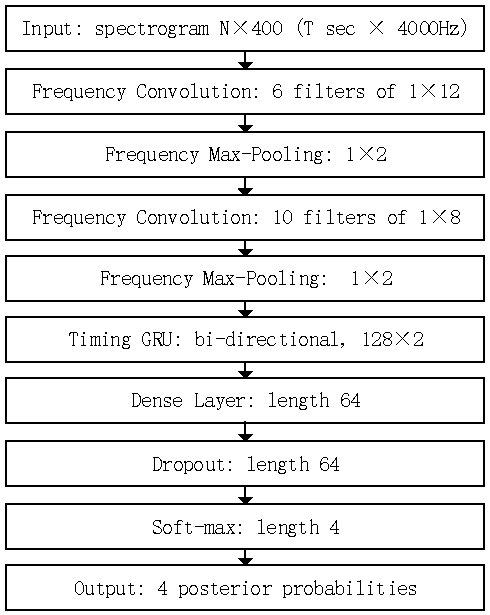
\includegraphics[height=10cm]{myfigures/var_len_nn_topology}
    \caption{深度神经网络结构}
    \label{fig:var_len_nn_topology}
\end{figure}

\subsection{实验结果}
\label{sec:var_len_experiement_result}

实验结果主要可以分为两个部分,第一部分主要比较了定长方法和本章的变长方法之间识别率的差异;第二部分主要通过图像来展示RNN不同节点在不同时间步的激活程度,从而进一步证明变长的方法可以减轻模型对于不同情感的混淆。

\subsubsection{准确率对比}
\label{sec:var_len_experiement_acc}
本次实验的评价指标仍然是加权准确率(Weighted Accuracy, WA)和不加权准确率(Unweighted Accuracy, UA),在下面的表\ref{tab:acc_var_len}中,我们展示了上一章定长方法取得的最好的结果,由于本章采用的网络结构和上一章不同,所以也会展示定长的输入在本章神经网络模型上的结果,以及变长的输入在本章神经网络上的结果,其中,“上一章最佳结果”代表上一章的最好的结果,“定长模型”和“变长模型”分别代表在本章设计的神经网络模型下定长输入和变长输入得到的结果。从实验结果中我们可以看出,当采用变长的神经网络结构时,相比于定长的方法,在WA和UA上均得到了提升,并且准确率超过了之前在IEMOCAP数据库上的最好结果(The State of Art)。这证明采用变长的输入比切分成定长的输入能够取得更好的效果。
\begin{table}[htb]
\centering
\begin{minipage}[t]{0.8\linewidth} % 如果想在表格中使用脚注,minipage是个不错的办法
\caption{不同方法的准确率}
\label{tab:acc_var_len}
    % \begin{tabular}{p{6cm}<{\centering} p{6cm}<{\centering}}
    \begin{tabularx}{\linewidth}{X<{\centering} X<{\centering} X<{\centering}}
        \toprule[1.5pt]
        模型 & WA & UA \\
        \midrule[1pt]
        上一章最佳结果 & 67.30\% & 62.00\% \\
        定长模型 & 68.86\% & 57.45\% \\
        变长模型 & \textbf{71.45\%} & \textbf{64.22\%} \\
        \bottomrule[1.5pt]
    \end{tabularx}
\end{minipage}
\end{table}

为了进一步分析实验结果,我们在下面的表格\ref{tab:cm_const_len}和表格\ref{tab:cm_var_len}中分别展示了定长输入和变长输入在本章的神经网络结构中得到的混淆矩阵。我们可以看到中性情感在变长方法的识别率提升了,正如我们在\ref{sec:var_len_intro}节分析的,当整个句子输入模型时可以减轻中性情感和其他情感的混淆。此外,高兴的准确率也得到了显著的提升,这或许是因为定长方法中,高兴句子切分出的语音段大多为中性情感,所以会被错分为其他情感。还有就是悲伤的识别率降低了,这或许是因为其他情感的准确率提升了,所以导致一些悲伤的语音被错分到其他情感。这些结果可以证明变长的方法确实能够提升部分情感的识别率。

\begin{table}[htb]
\centering
\begin{minipage}[t]{0.8\linewidth} % 如果想在表格中使用脚注,minipage是个不错的办法
\caption{混淆矩阵(定长输入)}
\label{tab:cm_const_len}
    % \begin{tabular}{p{6cm}<{\centering} p{6cm}<{\centering}}
    \begin{tabularx}{\linewidth}{X<{\centering} X<{\centering} X<{\centering} X<{\centering} X<{\centering}}
        \toprule[1.5pt]
        \diagbox[width=5em,trim=l]{实际}{预测} & 中性 & 愤怒 & 高兴 & 悲伤 \\
        \midrule[1pt]
        中性 & \textbf{71.75\%} & 8.88\% & 5.93\% & 13.45\% \\
        愤怒 & 30.84\% & \textbf{58.79\%} & 7.05\% & 3.34\% \\
        高兴 & 55.92\% & 31.42\% & \textbf{11.72\%} & 0.95\% \\
        悲伤 & 11.41\% & 0\% & 1.02\% & \textbf{87.57\%} \\
        \bottomrule[1.5pt]
    \end{tabularx}
\end{minipage}
\end{table}

\begin{table}[htb]
\centering
\begin{minipage}[t]{0.8\linewidth} % 如果想在表格中使用脚注,minipage是个不错的办法
\caption{混淆矩阵(变长输入)}
\label{tab:cm_var_len}
    % \begin{tabular}{p{6cm}<{\centering} p{6cm}<{\centering}}
    \begin{tabularx}{\linewidth}{X<{\centering} X<{\centering} X<{\centering} X<{\centering} X<{\centering}}
        \toprule[1.5pt]
        \diagbox[width=5em,trim=l]{实际}{预测} & 中性 & 愤怒 & 高兴 & 悲伤 \\
        \midrule[1pt]
        中性 & \textbf{73.64\%} & 2.74\% & 12.41\% & 11.21\% \\
        愤怒 & 11.44\% & \textbf{59.55\%} & 26.52\% & 2.5\% \\
        高兴 & 45.20\% & 13.81\% & \textbf{40.05\%} & 0.95\% \\
        悲伤 & 15.89\% & 0\% & 0.48\% & \textbf{83.64\%} \\
        \bottomrule[1.5pt]
    \end{tabularx}
\end{minipage}
\end{table}

\subsubsection{循环神经网络输出}
\label{sec:var_len_experiement_rnn}

通过观察神经网络的激活输出能够验证网络学习到的信息,下面的图\ref{fig:rnn_out_comp}展示了一个中性语音的句子通过神经网络后RNN不同节点的激活输出。左边的图片代表定长神经网络,右边的图片代表变长神经网络,其中横轴代表时间,纵轴代表RNN不同的节点,颜色越深代表激活程度越高。从图中可以观察到右边图片中的条纹比左边图片中的要清晰很多。条纹清晰代表RNN的每个节点没有混淆,明确知道应该在何种输入下激活,而条纹模糊代表节点无法清楚知道应该在何时激活,这也就是定长方法将中性语音段标记为其他情感类别来训练模型而导致的混淆。

\begin{figure}[h]
    \vspace{-0cm}  %调整图片与上文的垂直距离
    \setlength{\belowcaptionskip}{0cm}   %调整图片标题与下文距离
    \begin{minipage}{0.48\textwidth}
        \centering
        
\includegraphics[height=5cm]{myfigures/rnn_out_const_neu_comp}
        \centerline{(a) 定长方法}\medskip
    \end{minipage}\hfill
    \begin{minipage}{0.48\textwidth}
        \centering
        
\includegraphics[height=5cm]{myfigures/rnn_out_var_neu_comp}
        \centerline{(b) 变长方法}\medskip
    \end{minipage}
    \caption{同一句话在定长方法和变长方法中循环神经网络的激活输出}
    \label{fig:rnn_out_comp}
\end{figure}

此外,我们也发现特定的情感在特定的节点上有更高的激活值。图\ref{fig:rnn_out_ang}、图\ref{fig:rnn_out_hap}和图\ref{fig:rnn_out_sad}分别展示了三种不同情感的语音在变长网络中的RNN的不同节点的激活输出,红色方框中的是高激活度的节点,分别用数字为不同的红色框标号。从图中可以发现高兴和愤怒的激活节点比较相似,例如图\ref{fig:rnn_out_ang}的1、2、4号红色框的位置分别和图\ref{fig:rnn_out_hap}的1、2、5号红色框的位置很接近,这是因为高兴和愤怒的语音在声学表现上比较相似。然而,高兴的语音和悲伤的语音在声学表现上有很大的区别,所以这两种语音输入网络后的激活节点就有明显的不同。从图\ref{fig:rnn_out_hap}和图\ref{fig:rnn_out_sad}中可以看出,高兴语音和悲伤语音所代表的图中,红色框所在的位置大多数都不同。此外,中性情感无法找到特定的激活节点,这可能是因为中性语音没有一种特别明显的声学表现,所以也没有特定的激活节点。这些不同情感对应的激活节点可以在变长网络中清楚地观察到。但在定长网络中,RNN不同节点的输出都和图\ref{fig:rnn_out_comp}中(a)相似,其激活条纹非常模糊,所以导致很难观察到和变长网络中一样的激活节点。这些实验结果通过图像展示RNN不同节点的激活输出,进一步证明了变长的方法能够减轻模型对不同情感的混淆。

\begin{figure}[h] % use float package if you want it here
    \vspace{-0cm}  %调整图片与上文的垂直距离
    \setlength{\belowcaptionskip}{0cm}   %调整图片标题与下文距离
    \centering
    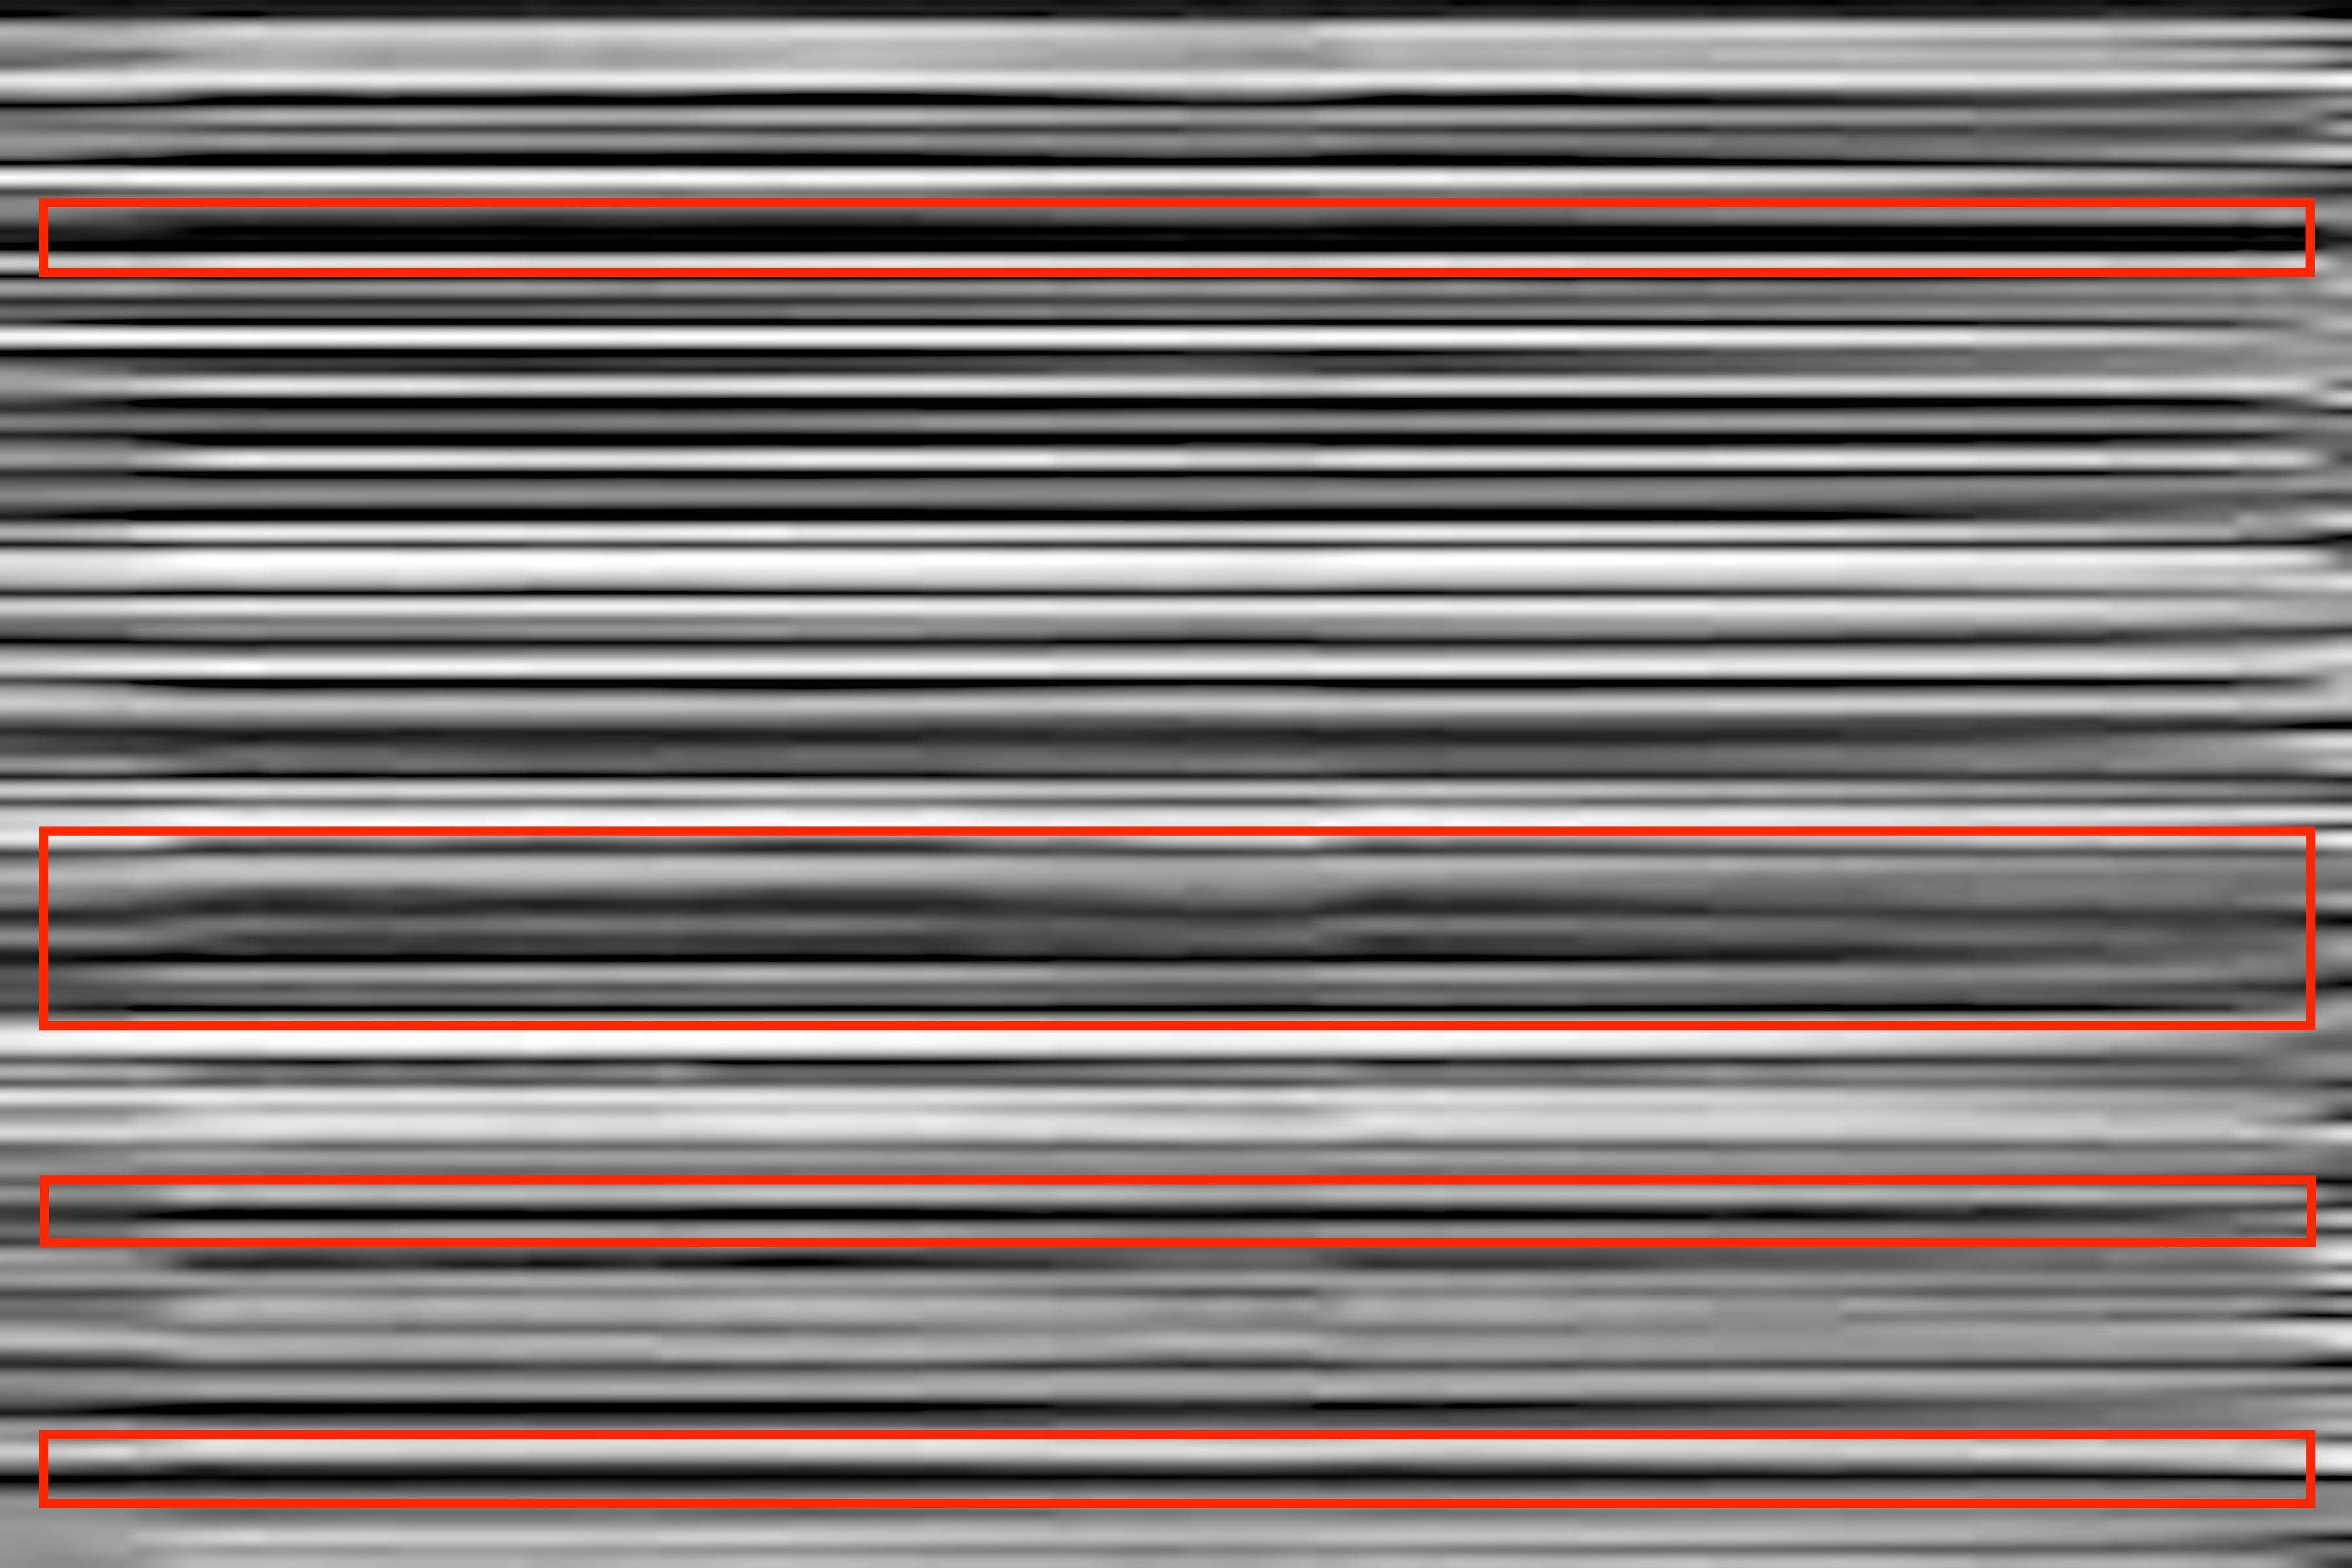
\includegraphics[height=7cm]{myfigures/rnn_out_var_ang}
    \caption{愤怒语音在变长循环神经网络上的激活输出}
    \label{fig:rnn_out_ang}
\end{figure}

\begin{figure}[h] % use float package if you want it here
    \vspace{-0.8cm}  %调整图片与上文的垂直距离 
    \setlength{\belowcaptionskip}{0cm}   %调整图片标题与下文距离
    \centering
    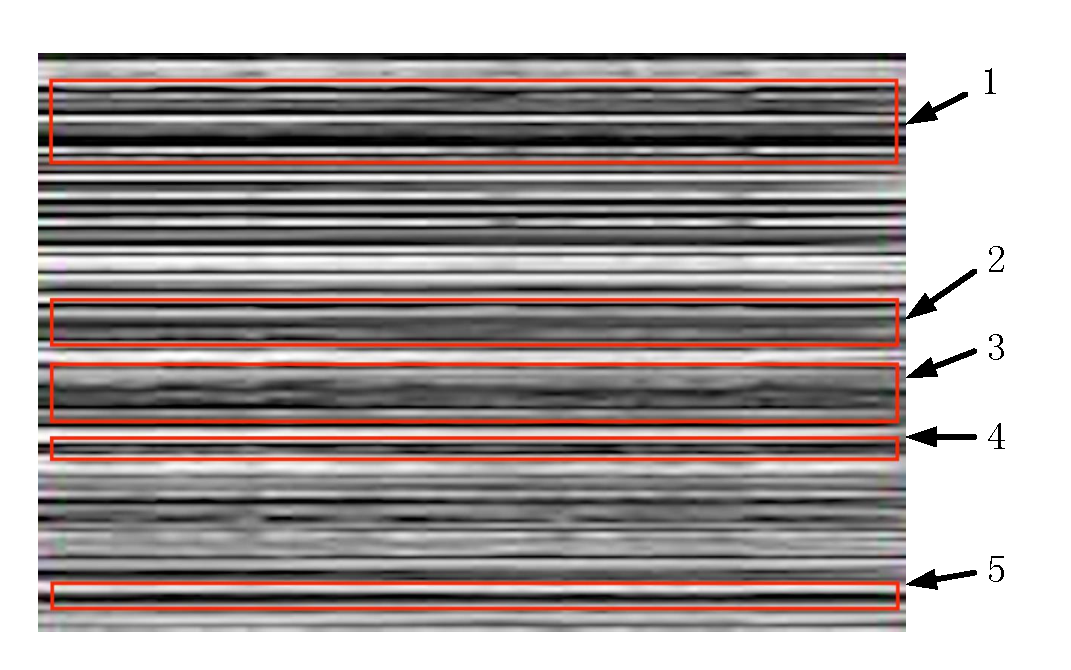
\includegraphics[height=7cm]{myfigures/rnn_out_var_hap}
    \caption{高兴语音在变长循环神经网络上的激活输出}
    \label{fig:rnn_out_hap}
\end{figure}

\begin{figure}[!tp] % use float package if you want it here
    \vspace{-0cm}  %调整图片与上文的垂直距离
    \setlength{\belowcaptionskip}{0cm}   %调整图片标题与下文距离
    \centering
    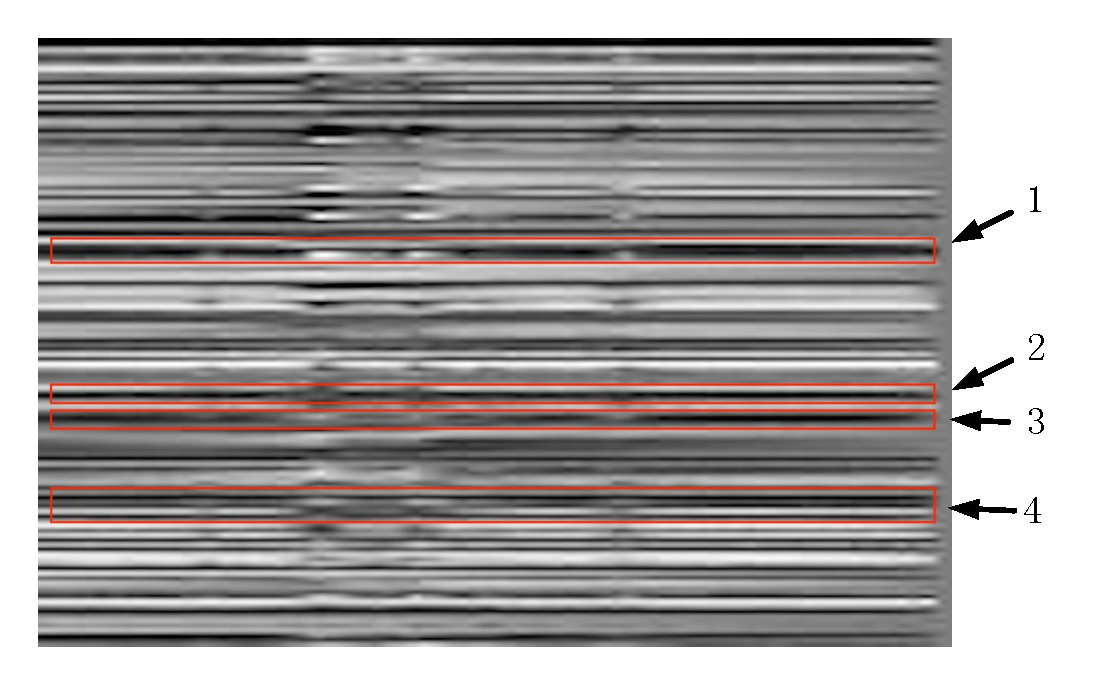
\includegraphics[height=7cm]{myfigures/rnn_out_var_sad}
    \caption{悲伤语音在变长循环神经网络上的激活输出}
    \label{fig:rnn_out_sad}
\end{figure}

% \begin{figure}[htb]
% \begin{minipage}{0.33\textwidth}
%     \centering
%     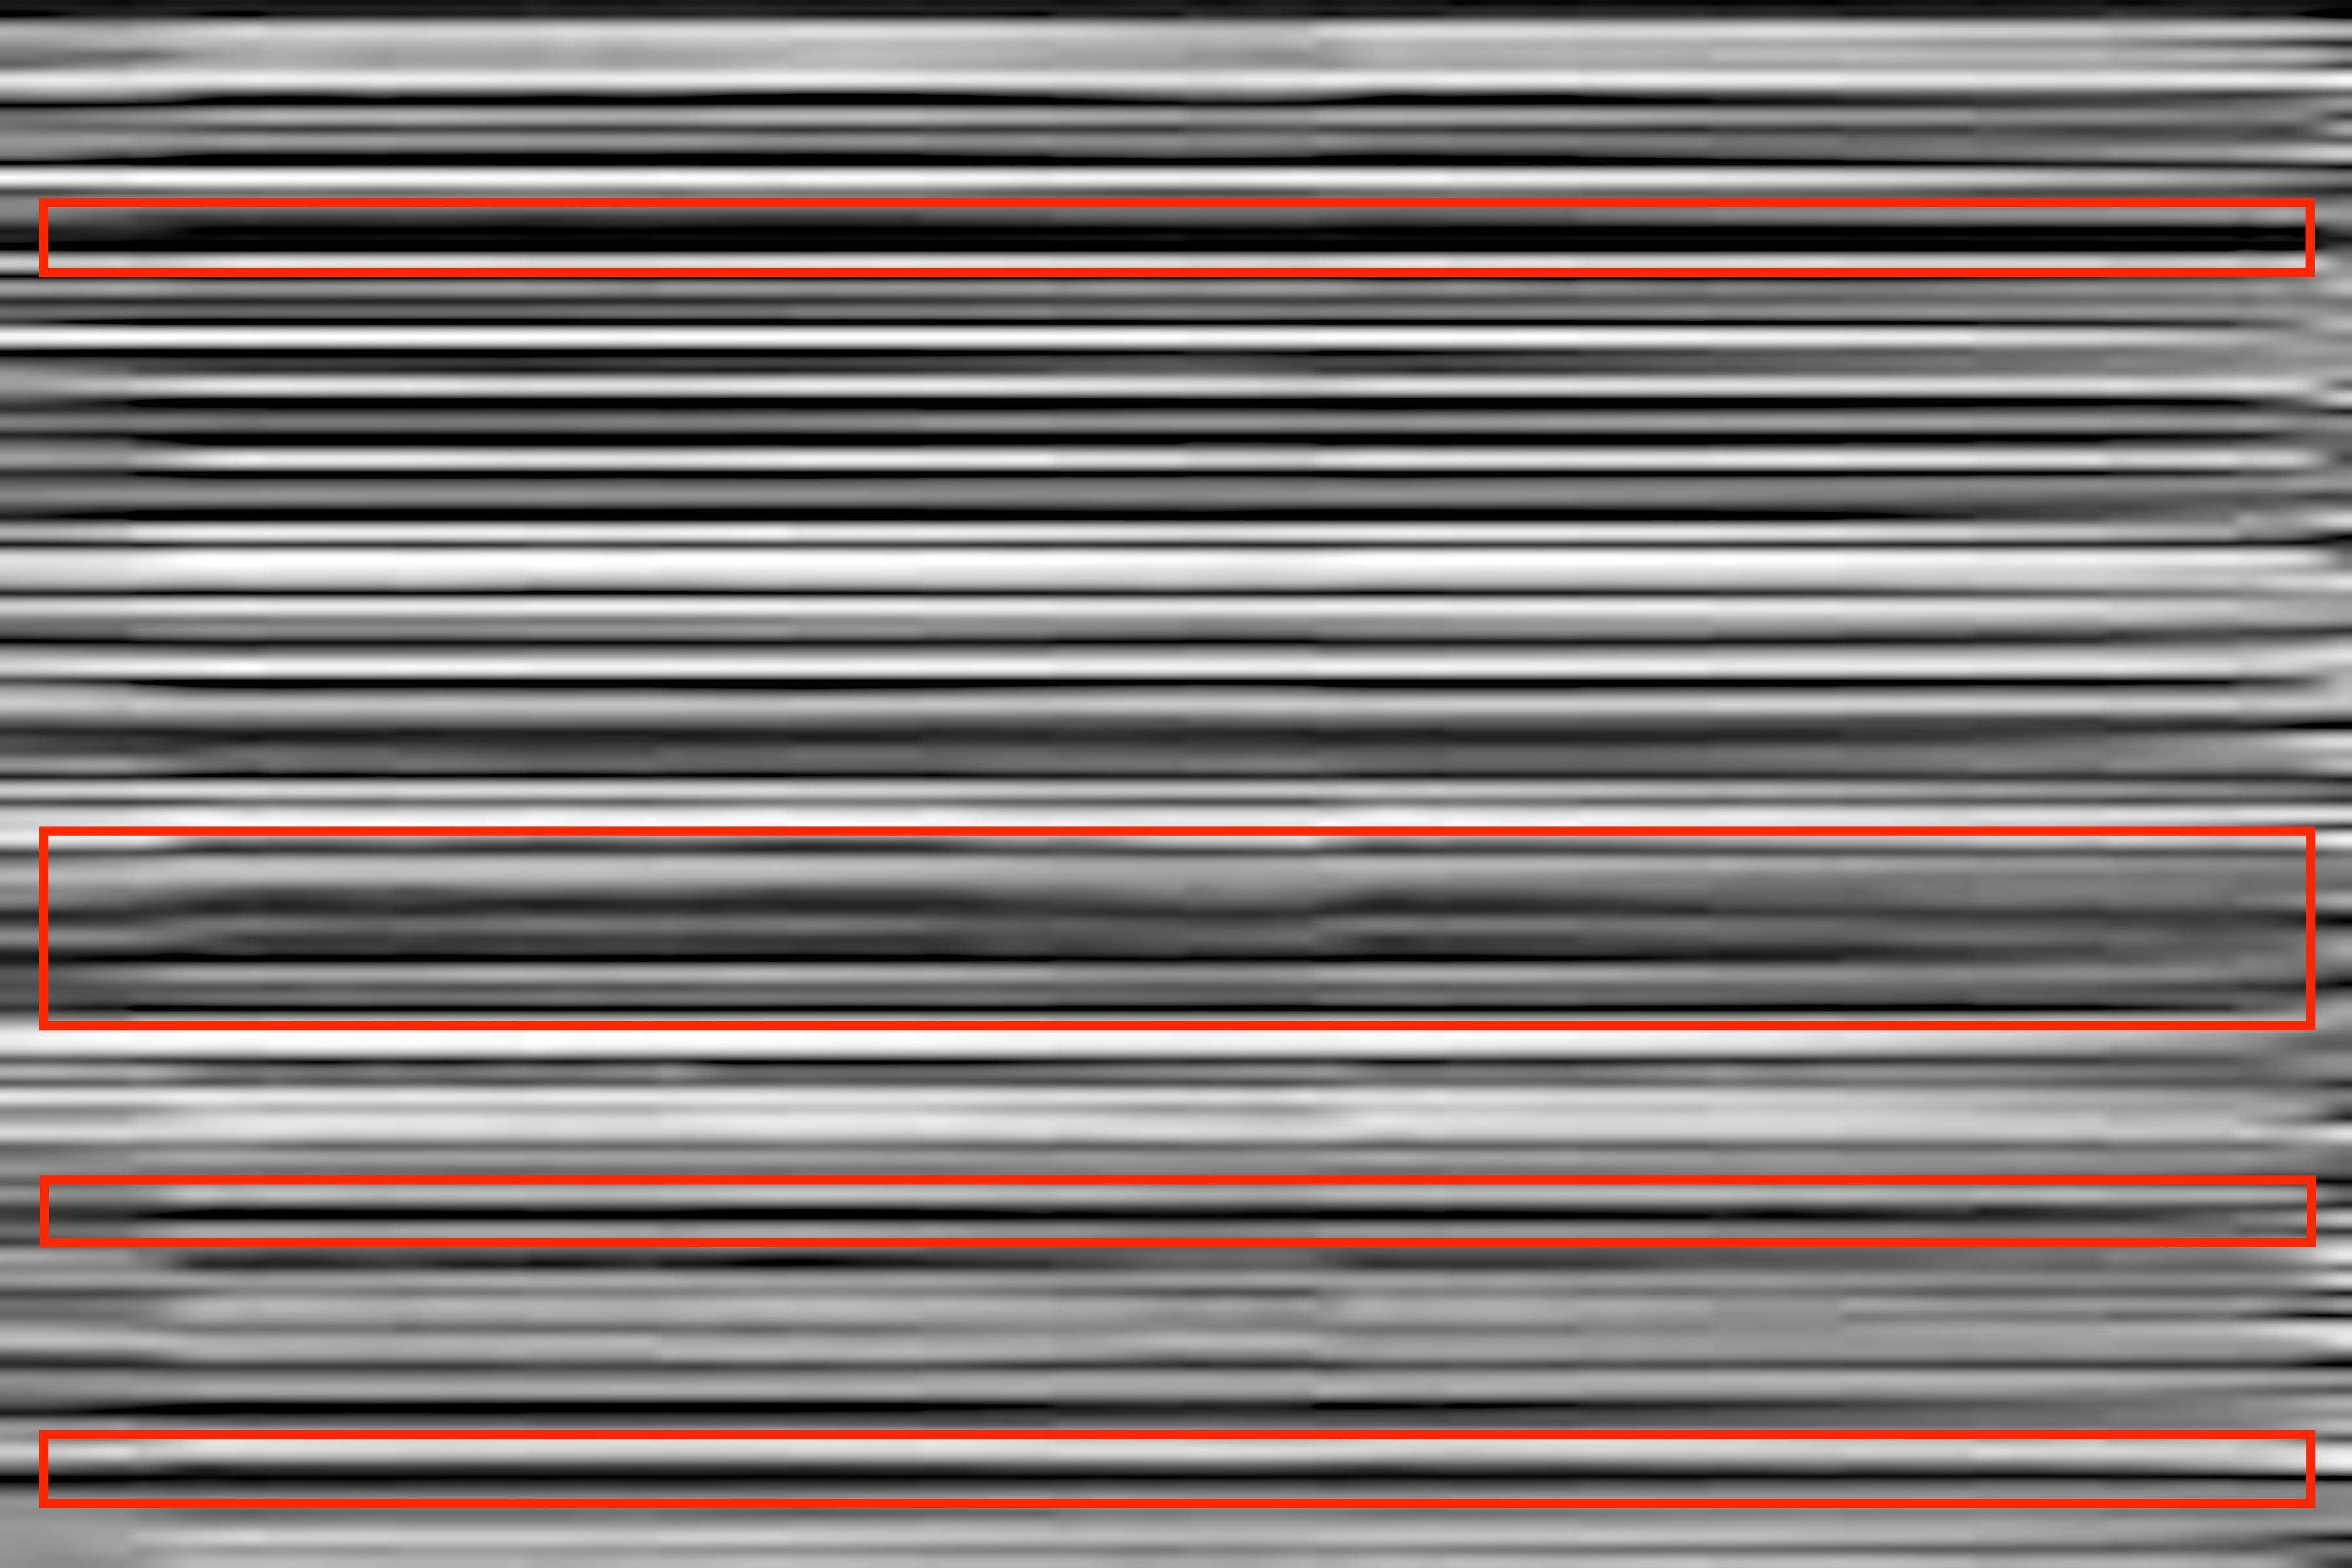
\includegraphics[height=3cm]{myfigures/rnn_out_var_ang}
%     \centerline{(a) 愤怒}\medskip
% \end{minipage}\hfill
% \begin{minipage}{0.33\textwidth}
%     \centering
%     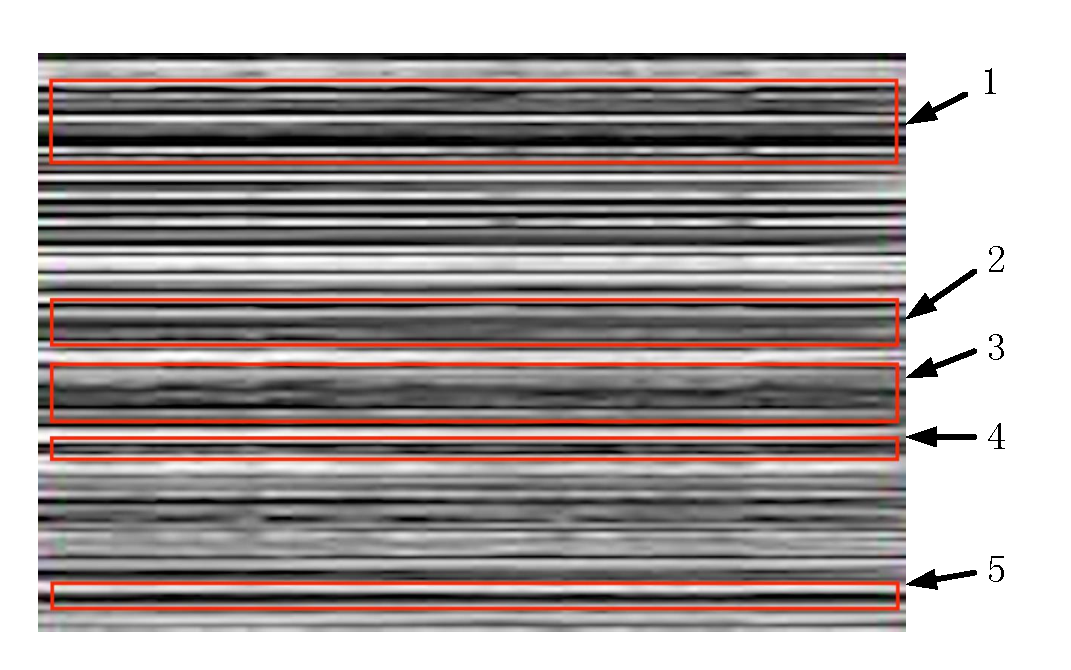
\includegraphics[height=3cm]{myfigures/rnn_out_var_hap}
%     \centerline{(b) 高兴}\medskip
% \end{minipage}
% \begin{minipage}{0.33\textwidth}
%     \centering
%     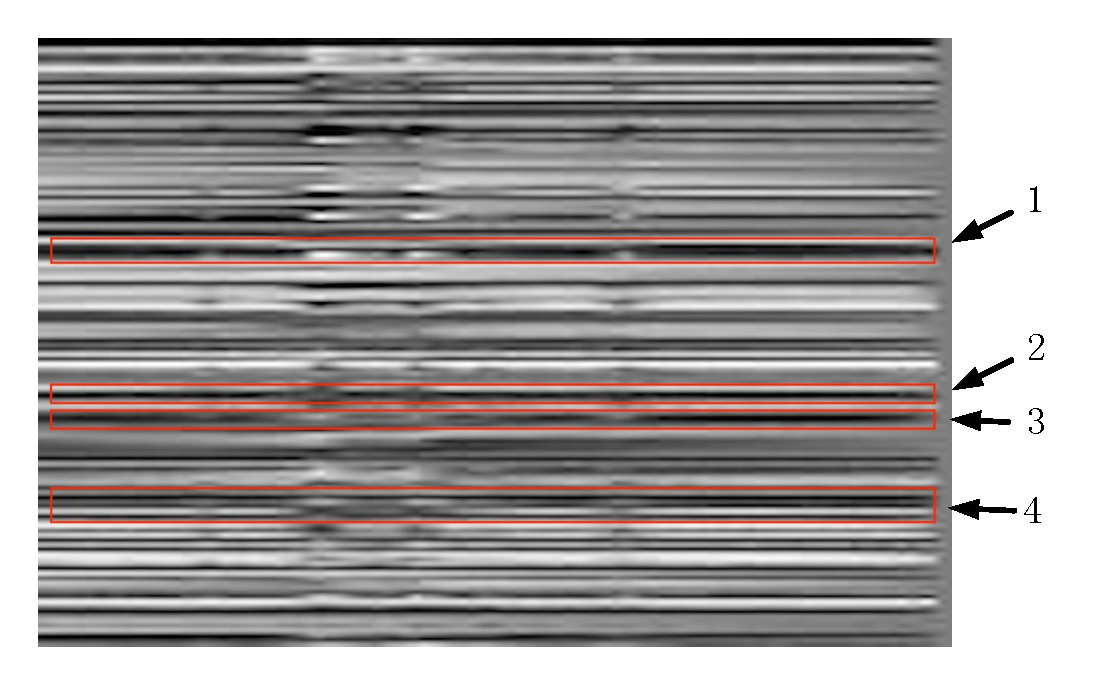
\includegraphics[height=3cm]{myfigures/rnn_out_var_sad}
%     \centerline{(c) 悲伤}\medskip
% \end{minipage}
% \caption{不同情感的语音在变长循环神经网络上的激活输出‘}
% \label{fig:rnn_out_emotions}
% \end{figure}

\section{本章小结}
\label{sec:var_len_summary}

本章主要设计了一种能够处理变长语音段输入的深度神经网络结构,相比于上一章提出的定长输入的深度神经网络模型,可以有效地减轻模型对不同情感的混淆。在情感语音数据库IEMOCAP上,变长的方法方法相比于定长的方法能够取得更好的识别率,并且超过了之前的最好结果(state-of-the-art)。